\newpage
\section{Versuchsaufbau}
\label{sec:Aufbau}

Ein Ausschnitt des nachfolgend beschriebenen Versuchsaufbaus
ist in Abbildung \ref{fig:aufbau} dargestellt.
Die Gamma-Strahlung einer \ce{^{137}Cs}
Quelle wird durch eine Blende kollimiert und trifft auf eine Probe in Form
eines Würfels.
Dabei verhindert die Kollimation eine Ausbreitung der Strahlung im Sinne
des Strahlenschutzes.
In Strahlrichtung hinter dem Würfel befindet sich ein NaJ-Detektor.
Von diesem Szintillationsdetektor werden Pulse erzeugt
und nach einer Verstärkung in einen Multichannelanalyser gegeben.
Diese Pulse werden durch Elektronen im Szintillator (hier NaJ) erzeugt,
indem einfallende Strahlung die Elektronen anregt und die Anregungsenergie
im Anschluss in Form von Photonen wieder abgegeben wird (indem die Elektronen
wieder auf niedrigere Energieniveaus fallen).
Im angeschlossenen Multichannelanalyser werden diese Pulse dann in ein
Energie-Zählrate-Histogramm übersetzt.
Dieser Analyser ist an einen Computer angeschlossen,
auf welchem mittels des Programms \texttt{MAESTRO}
das erstellte Histogramm ausgelesen und gespeichert wird.
Der Versuchsaufbau befindet sich mit Ausnahme des Computers hinter einem
Schutz aus Bleiklötzen, um eine Strahlungsaufnahme möglichst zu vermeiden.
Es werden die folgenden vier Proben verwendet:
Die erste Probe besteht aus einem hohlen würfelförmigen Aluminiumgehäuse.
Probe zwei und drei bestehen aus dem selben Aluminiumgehäuse, jedoch befindet
sich innerhalb jeweils ein zu bestimmendes Material.
Schließlich besteht die vierte Probe ebenfalls aus einem Aluminiumgehäuse,
in welchem neun kleine Würfel unbekannten Materials in drei Schichten
von jeweils drei mal drei Würfeln untergebracht sind.
Eine schematische Darstellung der mittleren Ebene der vierten Probe befindet sich
in Abbildung \ref{fig:aufbau} mit dem Titel \enquote{Aufsicht}.
Jede Probe wird vertikal so positioniert, dass die mittlere Ebene analysiert
werden kann (siehe Abbildung \ref{fig:aufbau} \enquote{Seitenansicht}).
Weiterhin ist der Probenhalter horizontal verschieb- und drehbar.

\begin{figure}
  \centering
  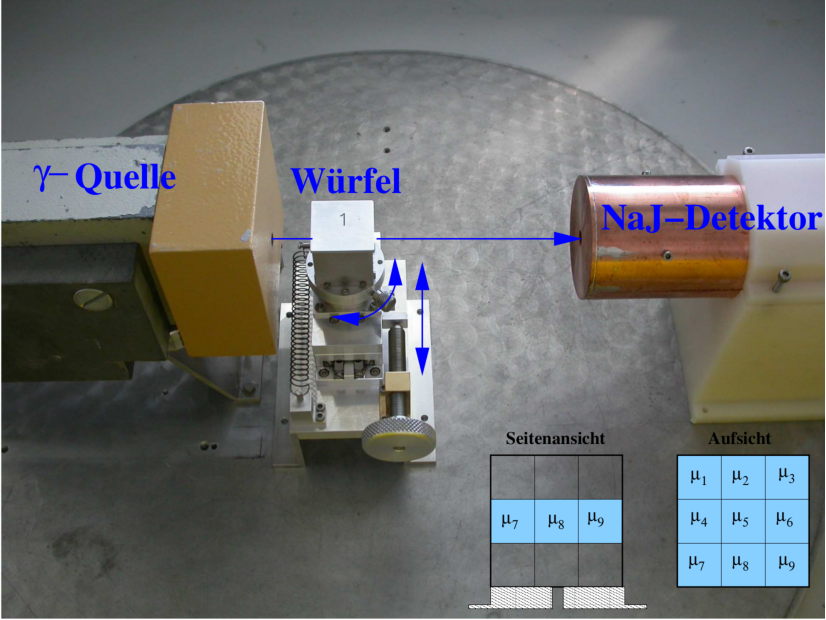
\includegraphics[height=8.0cm]{content/aufbau.pdf} % height=8.0cm
  \caption{Der verwendete Versuchsaufbau \cite[4]{anleitung}. In der unteren linken Ecke befinden
  sich zwei schematische Zeichnungen des vierten Würfels.}
  \label{fig:aufbau}
\end{figure}

\section{Durchführung}
\label{sec:Durchführung}

Im Programm \texttt{MAESTRO} werden für jede Messung die Marker so positionert,
dass nur der Photopeak des Sprektrums vermessen wird.
Der Photopeak hat wie in Abbildung \ref{fig:spektrum} beispielhaft dargestellt
die höchste Anzahl an Ereignissen im vermessenen Energiebereich, sodass
er sich zur Bestimmung der Absorptionskoeffizienten besonders gut eignet.
Nach dem Aufnehmen eines Spektrums
kann das Maximum des Photopeaks im Programm abgelesen werden.
Zu Beginn wird die Messzeit auf \SI{60}{\second} eingestellt und das Spektrum
der verwendeten Quelle ohne Probe vermessen. Im Anschluss werden die
Würfel \num{1} und \num{2} eingesetzt und bei einer Messzeit von
\SI{60}{\second} für Würfel \num{1} und \SI{480}{\second} für Würfel \num{2}
aus jeweils vier verschiedenen Positionen vermessen. Die Positionen sind
in Abbildung \ref{fig:wuerfelpos} als
$I_{1}, I_{2}, I_{11}$ und $I_{12}$ eingezeichnet.
Die Messzeit ist so zu wählen, dass die statistische Unsicherheit kleiner
als \SI{3}{\percent} ist, also im Photopeak mindestens circa \num{1112}
Ereignisse registriert werden.
Diese Anzahl an Ereignissen begründet sich auf der vorliegenden
Poissonverteilung der Ereignisse, sodass die statistische Unsicherheit
mit $1 / \sqrt{N}$ gegeben ist, wobei $N$ die Anzahl an Ereignissen darstellt.
Zuletzt wird Würfel vier eingesetzt und alle \num{12} in Abbildung
\ref{fig:wuerfelpos} dargestellten Strahlengänge werden vermessen. Dabei wird die
Messzeit auf \SI{480}{\second} eingestellt.

\begin{figure}
  \centering
  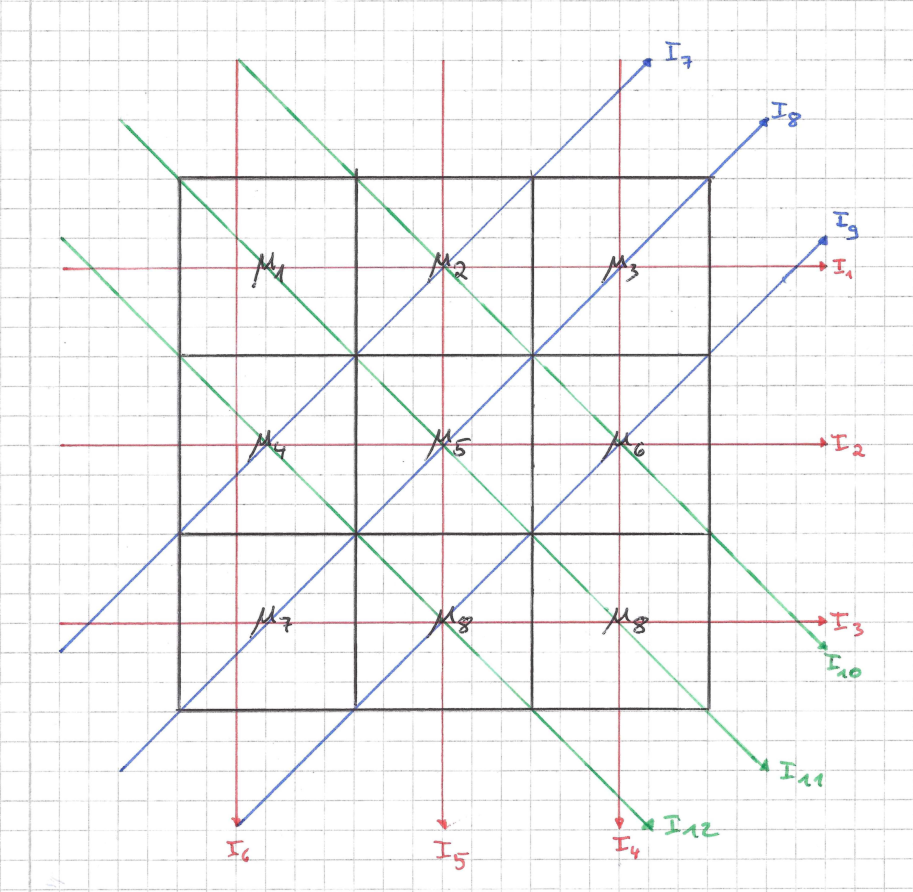
\includegraphics[height=8.0cm]{content/wuerfelpos.pdf} % height=8.0cm
  \caption{Die verschiedenen Strahlengänge durch die Würfelprobe.}
  \label{fig:wuerfelpos}
\end{figure}
